\documentclass[twoside]{book}

% Packages required by doxygen
\usepackage{fixltx2e}
\usepackage{calc}
\usepackage{doxygen}
\usepackage[export]{adjustbox} % also loads graphicx
\usepackage{graphicx}
\usepackage[utf8]{inputenc}
\usepackage{makeidx}
\usepackage{multicol}
\usepackage{multirow}
\PassOptionsToPackage{warn}{textcomp}
\usepackage{textcomp}
\usepackage[nointegrals]{wasysym}
\usepackage[table]{xcolor}

% Font selection
\usepackage[T1]{fontenc}
\usepackage[scaled=.90]{helvet}
\usepackage{courier}
\usepackage{amssymb}
\usepackage{sectsty}
\renewcommand{\familydefault}{\sfdefault}
\allsectionsfont{%
  \fontseries{bc}\selectfont%
  \color{darkgray}%
}
\renewcommand{\DoxyLabelFont}{%
  \fontseries{bc}\selectfont%
  \color{darkgray}%
}
\newcommand{\+}{\discretionary{\mbox{\scriptsize$\hookleftarrow$}}{}{}}

% Page & text layout
\usepackage{geometry}
\geometry{%
  a4paper,%
  top=2.5cm,%
  bottom=2.5cm,%
  left=2.5cm,%
  right=2.5cm%
}
\tolerance=750
\hfuzz=15pt
\hbadness=750
\setlength{\emergencystretch}{15pt}
\setlength{\parindent}{0cm}
\setlength{\parskip}{3ex plus 2ex minus 2ex}
\makeatletter
\renewcommand{\paragraph}{%
  \@startsection{paragraph}{4}{0ex}{-1.0ex}{1.0ex}{%
    \normalfont\normalsize\bfseries\SS@parafont%
  }%
}
\renewcommand{\subparagraph}{%
  \@startsection{subparagraph}{5}{0ex}{-1.0ex}{1.0ex}{%
    \normalfont\normalsize\bfseries\SS@subparafont%
  }%
}
\makeatother

% Headers & footers
\usepackage{fancyhdr}
\pagestyle{fancyplain}
\fancyhead[LE]{\fancyplain{}{\bfseries\thepage}}
\fancyhead[CE]{\fancyplain{}{}}
\fancyhead[RE]{\fancyplain{}{\bfseries\leftmark}}
\fancyhead[LO]{\fancyplain{}{\bfseries\rightmark}}
\fancyhead[CO]{\fancyplain{}{}}
\fancyhead[RO]{\fancyplain{}{\bfseries\thepage}}
\fancyfoot[LE]{\fancyplain{}{}}
\fancyfoot[CE]{\fancyplain{}{}}
\fancyfoot[RE]{\fancyplain{}{\bfseries\scriptsize Generated by Doxygen }}
\fancyfoot[LO]{\fancyplain{}{\bfseries\scriptsize Generated by Doxygen }}
\fancyfoot[CO]{\fancyplain{}{}}
\fancyfoot[RO]{\fancyplain{}{}}
\renewcommand{\footrulewidth}{0.4pt}
\renewcommand{\chaptermark}[1]{%
  \markboth{#1}{}%
}
\renewcommand{\sectionmark}[1]{%
  \markright{\thesection\ #1}%
}

% Indices & bibliography
\usepackage{natbib}
\usepackage[titles]{tocloft}
\setcounter{tocdepth}{3}
\setcounter{secnumdepth}{5}
\makeindex

% Hyperlinks (required, but should be loaded last)
\usepackage{ifpdf}
\ifpdf
  \usepackage[pdftex,pagebackref=true]{hyperref}
\else
  \usepackage[ps2pdf,pagebackref=true]{hyperref}
\fi
\hypersetup{%
  colorlinks=true,%
  linkcolor=blue,%
  citecolor=blue,%
  unicode%
}

% Custom commands
\newcommand{\clearemptydoublepage}{%
  \newpage{\pagestyle{empty}\cleardoublepage}%
}

\usepackage{caption}
\captionsetup{labelsep=space,justification=centering,font={bf},singlelinecheck=off,skip=4pt,position=top}

%===== C O N T E N T S =====

\begin{document}

% Titlepage & ToC
\hypersetup{pageanchor=false,
             bookmarksnumbered=true,
             pdfencoding=unicode
            }
\pagenumbering{alph}
\begin{titlepage}
\vspace*{7cm}
\begin{center}%
{\Large Julia Project }\\
\vspace*{1cm}
{\large Generated by Doxygen 1.8.13}\\
\end{center}
\end{titlepage}
\clearemptydoublepage
\pagenumbering{roman}
\tableofcontents
\clearemptydoublepage
\pagenumbering{arabic}
\hypersetup{pageanchor=true}

%--- Begin generated contents ---
\chapter{juliabrot \#}
\label{index}\hypertarget{index}{}\section*{level 1 header}

Julia set project description. 
\chapter{Hierarchical Index}
\section{Class Hierarchy}
This inheritance list is sorted roughly, but not completely, alphabetically\+:\begin{DoxyCompactList}
\item \contentsline{section}{Camera}{\pageref{classCamera}}{}
\item \contentsline{section}{Color\+Hsl}{\pageref{classColorHsl}}{}
\item \contentsline{section}{Julia\+Time}{\pageref{classJuliaTime}}{}
\item Q\+Main\+Window\begin{DoxyCompactList}
\item \contentsline{section}{Main\+Window}{\pageref{classMainWindow}}{}
\end{DoxyCompactList}
\item Q\+Object\begin{DoxyCompactList}
\item \contentsline{section}{Julia\+Renderer}{\pageref{classJuliaRenderer}}{}
\end{DoxyCompactList}
\item Q\+Widget\begin{DoxyCompactList}
\item \contentsline{section}{Julia\+Widget}{\pageref{classJuliaWidget}}{}
\end{DoxyCompactList}
\item \contentsline{section}{Vec2}{\pageref{classVec2}}{}
\end{DoxyCompactList}

\chapter{Class Index}
\section{Class List}
Here are the classes, structs, unions and interfaces with brief descriptions\+:\begin{DoxyCompactList}
\item\contentsline{section}{\hyperlink{classCamera}{Camera} \\*The \hyperlink{classCamera}{Camera} class }{\pageref{classCamera}}{}
\item\contentsline{section}{\hyperlink{classColorHsl}{Color\+Hsl} }{\pageref{classColorHsl}}{}
\item\contentsline{section}{\hyperlink{classJuliaRenderer}{Julia\+Renderer} }{\pageref{classJuliaRenderer}}{}
\item\contentsline{section}{\hyperlink{classJuliaTime}{Julia\+Time} }{\pageref{classJuliaTime}}{}
\item\contentsline{section}{\hyperlink{classJuliaWidget}{Julia\+Widget} }{\pageref{classJuliaWidget}}{}
\item\contentsline{section}{\hyperlink{classMainWindow}{Main\+Window} \\*Mainwindow include Qmainwindow }{\pageref{classMainWindow}}{}
\item\contentsline{section}{\hyperlink{classVec2}{Vec2} \\*(x,y) }{\pageref{classVec2}}{}
\end{DoxyCompactList}

\chapter{Class Documentation}
\hypertarget{classCamera}{}\section{Camera Class Reference}
\label{classCamera}\index{Camera@{Camera}}


The \hyperlink{classCamera}{Camera} class.  




{\ttfamily \#include $<$camera.\+h$>$}



Collaboration diagram for Camera\+:
\nopagebreak
\begin{figure}[H]
\begin{center}
\leavevmode
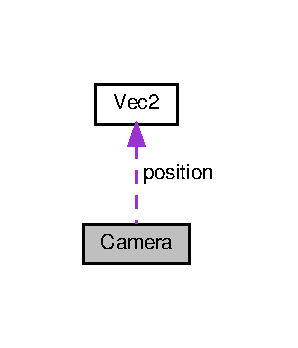
\includegraphics[width=143pt]{classCamera__coll__graph}
\end{center}
\end{figure}
\subsection*{Public Member Functions}
\begin{DoxyCompactItemize}
\item 
\mbox{\Hypertarget{classCamera_a01f94c3543f56ede7af49dc778f19331}\label{classCamera_a01f94c3543f56ede7af49dc778f19331}} 
\hyperlink{classCamera_a01f94c3543f56ede7af49dc778f19331}{Camera} ()
\begin{DoxyCompactList}\small\item\em \hyperlink{classCamera}{Camera} constructor. \end{DoxyCompactList}\end{DoxyCompactItemize}
\subsection*{Public Attributes}
\begin{DoxyCompactItemize}
\item 
\mbox{\Hypertarget{classCamera_a3d0e40ef5f4f22a013991bc46603c16b}\label{classCamera_a3d0e40ef5f4f22a013991bc46603c16b}} 
\hyperlink{classVec2}{Vec2} \hyperlink{classCamera_a3d0e40ef5f4f22a013991bc46603c16b}{position}
\begin{DoxyCompactList}\small\item\em position variable with datatype vec2 \end{DoxyCompactList}\item 
\mbox{\Hypertarget{classCamera_a3b777eab5439277827678d7aeb95315b}\label{classCamera_a3b777eab5439277827678d7aeb95315b}} 
double \hyperlink{classCamera_a3b777eab5439277827678d7aeb95315b}{zoom}
\begin{DoxyCompactList}\small\item\em zoom variable with type double \end{DoxyCompactList}\item 
\mbox{\Hypertarget{classCamera_a15c8b64066eda81920a6eac3cc8b86ca}\label{classCamera_a15c8b64066eda81920a6eac3cc8b86ca}} 
double \hyperlink{classCamera_a15c8b64066eda81920a6eac3cc8b86ca}{rotation}
\begin{DoxyCompactList}\small\item\em zoom variable with type double \end{DoxyCompactList}\end{DoxyCompactItemize}


\subsection{Detailed Description}
The \hyperlink{classCamera}{Camera} class. 

The documentation for this class was generated from the following files\+:\begin{DoxyCompactItemize}
\item 
camera.\+h\item 
camera.\+cpp\end{DoxyCompactItemize}

\hypertarget{classColorHsl}{}\section{Color\+Hsl Class Reference}
\label{classColorHsl}\index{Color\+Hsl@{Color\+Hsl}}


The \hyperlink{classColorHsl}{Color\+Hsl} class.  




{\ttfamily \#include $<$colorhsl.\+h$>$}

\subsection*{Static Public Member Functions}
\begin{DoxyCompactItemize}
\item 
static unsigned int \hyperlink{classColorHsl_ae9451e6216d6e40eb1d0754e580f4b01}{Get\+Rgb\+Uint32} (float h, float s, float l)
\end{DoxyCompactItemize}
\subsection*{Static Protected Member Functions}
\begin{DoxyCompactItemize}
\item 
static float \hyperlink{classColorHsl_ae5ee64095d7aaebb01498de2180daa9f}{Hue\+To\+Rgb} (float p, float q, float t)
\begin{DoxyCompactList}\small\item\em Hue\+To\+Rgb convert hue to rgb (used for hsl-\/2-\/rgb algorithm) \end{DoxyCompactList}\item 
static float \hyperlink{classColorHsl_a891b3f489be291ab418bffd0cc48f0ee}{Wrap\+Hue} (float hue)
\begin{DoxyCompactList}\small\item\em Wrap\+Hue wrap hue between 0 and 1. \end{DoxyCompactList}\end{DoxyCompactItemize}


\subsection{Detailed Description}
The \hyperlink{classColorHsl}{Color\+Hsl} class. 

\subsection{Member Function Documentation}
\mbox{\Hypertarget{classColorHsl_ae9451e6216d6e40eb1d0754e580f4b01}\label{classColorHsl_ae9451e6216d6e40eb1d0754e580f4b01}} 
\index{Color\+Hsl@{Color\+Hsl}!Get\+Rgb\+Uint32@{Get\+Rgb\+Uint32}}
\index{Get\+Rgb\+Uint32@{Get\+Rgb\+Uint32}!Color\+Hsl@{Color\+Hsl}}
\subsubsection{\texorpdfstring{Get\+Rgb\+Uint32()}{GetRgbUint32()}}
{\footnotesize\ttfamily unsigned int Color\+Hsl\+::\+Get\+Rgb\+Uint32 (\begin{DoxyParamCaption}\item[{float}]{h,  }\item[{float}]{s,  }\item[{float}]{l }\end{DoxyParamCaption})\hspace{0.3cm}{\ttfamily [static]}}

convert color from H\+SL to 32-\/bit integer (e.\+g. yellow = 0x\+F\+F\+F\+F00) 
\begin{DoxyParams}{Parameters}
{\em h} & hue from 0 to 1 \\
\hline
{\em s} & saturation from 0 to 1 \\
\hline
{\em l} & lightness from 0 to 1 \\
\hline
\end{DoxyParams}
\begin{DoxyReturn}{Returns}
32-\/bit integer (e.\+g. yellow = 0x\+F\+F\+F\+F00) 
\end{DoxyReturn}
\mbox{\Hypertarget{classColorHsl_ae5ee64095d7aaebb01498de2180daa9f}\label{classColorHsl_ae5ee64095d7aaebb01498de2180daa9f}} 
\index{Color\+Hsl@{Color\+Hsl}!Hue\+To\+Rgb@{Hue\+To\+Rgb}}
\index{Hue\+To\+Rgb@{Hue\+To\+Rgb}!Color\+Hsl@{Color\+Hsl}}
\subsubsection{\texorpdfstring{Hue\+To\+Rgb()}{HueToRgb()}}
{\footnotesize\ttfamily float Color\+Hsl\+::\+Hue\+To\+Rgb (\begin{DoxyParamCaption}\item[{float}]{p,  }\item[{float}]{q,  }\item[{float}]{t }\end{DoxyParamCaption})\hspace{0.3cm}{\ttfamily [static]}, {\ttfamily [protected]}}



Hue\+To\+Rgb convert hue to rgb (used for hsl-\/2-\/rgb algorithm) 


\begin{DoxyParams}{Parameters}
{\em p} & \\
\hline
{\em q} & \\
\hline
{\em t} & \\
\hline
\end{DoxyParams}
\begin{DoxyReturn}{Returns}

\end{DoxyReturn}
\mbox{\Hypertarget{classColorHsl_a891b3f489be291ab418bffd0cc48f0ee}\label{classColorHsl_a891b3f489be291ab418bffd0cc48f0ee}} 
\index{Color\+Hsl@{Color\+Hsl}!Wrap\+Hue@{Wrap\+Hue}}
\index{Wrap\+Hue@{Wrap\+Hue}!Color\+Hsl@{Color\+Hsl}}
\subsubsection{\texorpdfstring{Wrap\+Hue()}{WrapHue()}}
{\footnotesize\ttfamily float Color\+Hsl\+::\+Wrap\+Hue (\begin{DoxyParamCaption}\item[{float}]{hue }\end{DoxyParamCaption})\hspace{0.3cm}{\ttfamily [static]}, {\ttfamily [protected]}}



Wrap\+Hue wrap hue between 0 and 1. 


\begin{DoxyParams}{Parameters}
{\em hue} & \\
\hline
\end{DoxyParams}
\begin{DoxyReturn}{Returns}

\end{DoxyReturn}


The documentation for this class was generated from the following files\+:\begin{DoxyCompactItemize}
\item 
colorhsl.\+h\item 
colorhsl.\+cpp\end{DoxyCompactItemize}

\hypertarget{classJuliaRenderer}{}\section{Julia\+Renderer Class Reference}
\label{classJuliaRenderer}\index{Julia\+Renderer@{Julia\+Renderer}}


Collaboration diagram for Julia\+Renderer\+:
\nopagebreak
\begin{figure}[H]
\begin{center}
\leavevmode
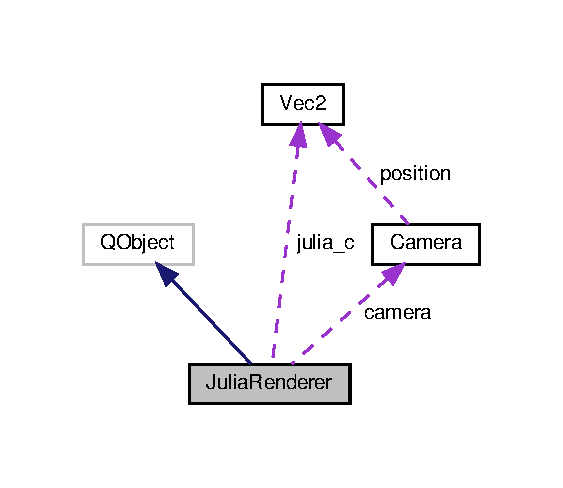
\includegraphics[width=270pt]{classJuliaRenderer__coll__graph}
\end{center}
\end{figure}
\subsection*{Public Member Functions}
\begin{DoxyCompactItemize}
\item 
\mbox{\Hypertarget{classJuliaRenderer_a6fc0f5a07835264e53ba7dea9a6562a4}\label{classJuliaRenderer_a6fc0f5a07835264e53ba7dea9a6562a4}} 
\hyperlink{classJuliaRenderer_a6fc0f5a07835264e53ba7dea9a6562a4}{Julia\+Renderer} ()
\begin{DoxyCompactList}\small\item\em default constructor \end{DoxyCompactList}\item 
\mbox{\Hypertarget{classJuliaRenderer_affd048fa174855e27db9453eda38d2ba}\label{classJuliaRenderer_affd048fa174855e27db9453eda38d2ba}} 
void \hyperlink{classJuliaRenderer_affd048fa174855e27db9453eda38d2ba}{update} ()
\begin{DoxyCompactList}\small\item\em update renderer updates camera position, colors, etc \end{DoxyCompactList}\item 
void \hyperlink{classJuliaRenderer_a2231caba8e65e19eb3074670c96e705f}{render} (Q\+Image \&image, double scale\+\_\+factor)
\begin{DoxyCompactList}\small\item\em render julia-\/set to image \end{DoxyCompactList}\end{DoxyCompactItemize}
\subsection*{Public Attributes}
\begin{DoxyCompactItemize}
\item 
\mbox{\Hypertarget{classJuliaRenderer_a273cae2c0c14f6bddc6196b46928d7bb}\label{classJuliaRenderer_a273cae2c0c14f6bddc6196b46928d7bb}} 
\hyperlink{classCamera}{Camera} \hyperlink{classJuliaRenderer_a273cae2c0c14f6bddc6196b46928d7bb}{camera}
\begin{DoxyCompactList}\small\item\em \hyperlink{classCamera}{Camera}, determines position, rotation and zoom of render. \end{DoxyCompactList}\item 
\mbox{\Hypertarget{classJuliaRenderer_a25369c5dcd4e85a6ee45413b46f59fef}\label{classJuliaRenderer_a25369c5dcd4e85a6ee45413b46f59fef}} 
\hyperlink{classVec2}{Vec2} \hyperlink{classJuliaRenderer_a25369c5dcd4e85a6ee45413b46f59fef}{julia\+\_\+c} = \hyperlink{classVec2}{Vec2}(0, 0)
\begin{DoxyCompactList}\small\item\em constant \textquotesingle{}c\textquotesingle{} for julia-\/set \end{DoxyCompactList}\item 
\mbox{\Hypertarget{classJuliaRenderer_ab2fb36d542bb5e630826cbfdcdfa6d00}\label{classJuliaRenderer_ab2fb36d542bb5e630826cbfdcdfa6d00}} 
int \hyperlink{classJuliaRenderer_ab2fb36d542bb5e630826cbfdcdfa6d00}{rendering\+\_\+mode} = 0
\begin{DoxyCompactList}\small\item\em set to 0 julia-\/set, 1 for mandelbrot \end{DoxyCompactList}\item 
\mbox{\Hypertarget{classJuliaRenderer_abf1c76861597558bd3b53d5f89c5d94e}\label{classJuliaRenderer_abf1c76861597558bd3b53d5f89c5d94e}} 
int \hyperlink{classJuliaRenderer_abf1c76861597558bd3b53d5f89c5d94e}{max\+\_\+iterations} = 25
\begin{DoxyCompactList}\small\item\em maximum number of iterations \end{DoxyCompactList}\item 
\mbox{\Hypertarget{classJuliaRenderer_a9e2d7418901019e060bb8cc9e0e9982d}\label{classJuliaRenderer_a9e2d7418901019e060bb8cc9e0e9982d}} 
int \hyperlink{classJuliaRenderer_a9e2d7418901019e060bb8cc9e0e9982d}{color\+\_\+mode} = 1
\begin{DoxyCompactList}\small\item\em determines how the fractal gets colorized \end{DoxyCompactList}\end{DoxyCompactItemize}
\subsection*{Protected Member Functions}
\begin{DoxyCompactItemize}
\item 
\mbox{\Hypertarget{classJuliaRenderer_a21a8248c28cf0035a14ad1ef98761356}\label{classJuliaRenderer_a21a8248c28cf0035a14ad1ef98761356}} 
bool {\bfseries event\+Filter} (Q\+Object $\ast$Obj, Q\+Event $\ast$event) override
\end{DoxyCompactItemize}


\subsection{Member Function Documentation}
\mbox{\Hypertarget{classJuliaRenderer_a2231caba8e65e19eb3074670c96e705f}\label{classJuliaRenderer_a2231caba8e65e19eb3074670c96e705f}} 
\index{Julia\+Renderer@{Julia\+Renderer}!render@{render}}
\index{render@{render}!Julia\+Renderer@{Julia\+Renderer}}
\subsubsection{\texorpdfstring{render()}{render()}}
{\footnotesize\ttfamily void Julia\+Renderer\+::render (\begin{DoxyParamCaption}\item[{Q\+Image \&}]{image,  }\item[{double}]{scale\+\_\+factor }\end{DoxyParamCaption})}



render julia-\/set to image 


\begin{DoxyParams}{Parameters}
{\em image} & the image to render the julia-\/set to \\
\hline
{\em scale\+\_\+factor} & multiplicator for camera.\+zoom, used to keep zoom consistent for different quality settings \\
\hline
\end{DoxyParams}


The documentation for this class was generated from the following files\+:\begin{DoxyCompactItemize}
\item 
juliarenderer.\+h\item 
juliarenderer.\+cpp\end{DoxyCompactItemize}

\hypertarget{classJuliaTime}{}\section{Julia\+Time Class Reference}
\label{classJuliaTime}\index{Julia\+Time@{Julia\+Time}}
\subsection*{Static Public Member Functions}
\begin{DoxyCompactItemize}
\item 
\mbox{\Hypertarget{classJuliaTime_a0de18abd49917adc503f1065aa1e47b4}\label{classJuliaTime_a0de18abd49917adc503f1065aa1e47b4}} 
static void \hyperlink{classJuliaTime_a0de18abd49917adc503f1065aa1e47b4}{update} ()
\begin{DoxyCompactList}\small\item\em update time (recalculates time since start, delta time, fps, etc) \end{DoxyCompactList}\item 
\mbox{\Hypertarget{classJuliaTime_ae466da8414d593da71a955e0bcd2b816}\label{classJuliaTime_ae466da8414d593da71a955e0bcd2b816}} 
static void \hyperlink{classJuliaTime_ae466da8414d593da71a955e0bcd2b816}{start} ()
\begin{DoxyCompactList}\small\item\em start time (initialize everything) \end{DoxyCompactList}\end{DoxyCompactItemize}
\subsection*{Static Public Attributes}
\begin{DoxyCompactItemize}
\item 
\mbox{\Hypertarget{classJuliaTime_ada9446882532931111011695d7ed2e02}\label{classJuliaTime_ada9446882532931111011695d7ed2e02}} 
static int \hyperlink{classJuliaTime_ada9446882532931111011695d7ed2e02}{start\+Time\+Ms} = 0
\begin{DoxyCompactList}\small\item\em start timestamp (in ms) \end{DoxyCompactList}\item 
\mbox{\Hypertarget{classJuliaTime_a843524b27f79699732a64dabde8992d5}\label{classJuliaTime_a843524b27f79699732a64dabde8992d5}} 
static int \hyperlink{classJuliaTime_a843524b27f79699732a64dabde8992d5}{current\+Time\+Ms} = 0
\begin{DoxyCompactList}\small\item\em timestamp current (in ms) \end{DoxyCompactList}\item 
\mbox{\Hypertarget{classJuliaTime_aeda4f6b158bbca7f22acb28020ba9891}\label{classJuliaTime_aeda4f6b158bbca7f22acb28020ba9891}} 
static int \hyperlink{classJuliaTime_aeda4f6b158bbca7f22acb28020ba9891}{last\+Time\+Ms} = 0
\begin{DoxyCompactList}\small\item\em timestamp from last update (in ms) \end{DoxyCompactList}\item 
\mbox{\Hypertarget{classJuliaTime_a3a9b7d1156c8fc6ca35d52cc90f2324a}\label{classJuliaTime_a3a9b7d1156c8fc6ca35d52cc90f2324a}} 
static int \hyperlink{classJuliaTime_a3a9b7d1156c8fc6ca35d52cc90f2324a}{delta\+Time\+Ms} = 0
\begin{DoxyCompactList}\small\item\em time passed since last update (in ms) \end{DoxyCompactList}\item 
\mbox{\Hypertarget{classJuliaTime_a55613ba6095a84edae7de90b6c2c16a5}\label{classJuliaTime_a55613ba6095a84edae7de90b6c2c16a5}} 
static double \hyperlink{classJuliaTime_a55613ba6095a84edae7de90b6c2c16a5}{since\+Start} = 0.\+0
\begin{DoxyCompactList}\small\item\em time passed since start (in seconds) \end{DoxyCompactList}\item 
\mbox{\Hypertarget{classJuliaTime_a9bc0d5c43e2bfbefd25ff742d9aa3042}\label{classJuliaTime_a9bc0d5c43e2bfbefd25ff742d9aa3042}} 
static double \hyperlink{classJuliaTime_a9bc0d5c43e2bfbefd25ff742d9aa3042}{delta\+Time} = 0.\+0
\begin{DoxyCompactList}\small\item\em time passed since last update (in seconds) \end{DoxyCompactList}\item 
\mbox{\Hypertarget{classJuliaTime_ad2bffc176fa8c7d97e95459631d739d8}\label{classJuliaTime_ad2bffc176fa8c7d97e95459631d739d8}} 
static int \hyperlink{classJuliaTime_ad2bffc176fa8c7d97e95459631d739d8}{fps} = 0
\begin{DoxyCompactList}\small\item\em current fps (updates every second) \end{DoxyCompactList}\end{DoxyCompactItemize}


The documentation for this class was generated from the following files\+:\begin{DoxyCompactItemize}
\item 
juliatime.\+h\item 
juliatime.\+cpp\end{DoxyCompactItemize}

\hypertarget{classJuliaWidget}{}\section{Julia\+Widget Class Reference}
\label{classJuliaWidget}\index{Julia\+Widget@{Julia\+Widget}}


Collaboration diagram for Julia\+Widget\+:
\nopagebreak
\begin{figure}[H]
\begin{center}
\leavevmode
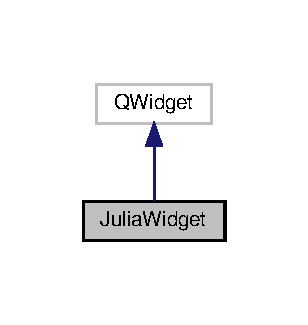
\includegraphics[width=148pt]{classJuliaWidget__coll__graph}
\end{center}
\end{figure}
\subsection*{Public Member Functions}
\begin{DoxyCompactItemize}
\item 
\mbox{\Hypertarget{classJuliaWidget_a43281a37bd560567372d1f9ccfd673c5}\label{classJuliaWidget_a43281a37bd560567372d1f9ccfd673c5}} 
{\bfseries Julia\+Widget} (Q\+Widget $\ast$parent=nullptr)
\item 
void \hyperlink{classJuliaWidget_a686d58acadb8eaa396ca6904318a5547}{set\+Image} (Q\+Image $\ast$\hyperlink{classJuliaWidget_abc96ffcb51d90cc16ed92242fdb62d1b}{image})
\end{DoxyCompactItemize}
\subsection*{Protected Member Functions}
\begin{DoxyCompactItemize}
\item 
\mbox{\Hypertarget{classJuliaWidget_a65d06d3f69873f573380fde577abfcf2}\label{classJuliaWidget_a65d06d3f69873f573380fde577abfcf2}} 
void {\bfseries paint\+Event} (Q\+Paint\+Event $\ast$event)
\end{DoxyCompactItemize}
\subsection*{Protected Attributes}
\begin{DoxyCompactItemize}
\item 
\mbox{\Hypertarget{classJuliaWidget_abc96ffcb51d90cc16ed92242fdb62d1b}\label{classJuliaWidget_abc96ffcb51d90cc16ed92242fdb62d1b}} 
Q\+Image $\ast$ \hyperlink{classJuliaWidget_abc96ffcb51d90cc16ed92242fdb62d1b}{image}
\begin{DoxyCompactList}\small\item\em the image to draw to the panel \end{DoxyCompactList}\end{DoxyCompactItemize}


\subsection{Member Function Documentation}
\mbox{\Hypertarget{classJuliaWidget_a686d58acadb8eaa396ca6904318a5547}\label{classJuliaWidget_a686d58acadb8eaa396ca6904318a5547}} 
\index{Julia\+Widget@{Julia\+Widget}!set\+Image@{set\+Image}}
\index{set\+Image@{set\+Image}!Julia\+Widget@{Julia\+Widget}}
\subsubsection{\texorpdfstring{set\+Image()}{setImage()}}
{\footnotesize\ttfamily void Julia\+Widget\+::set\+Image (\begin{DoxyParamCaption}\item[{Q\+Image $\ast$}]{image }\end{DoxyParamCaption})}

set the image that gets renderer to the widget panel 
\begin{DoxyParams}{Parameters}
{\em image} & pointer to the image \\
\hline
\end{DoxyParams}


The documentation for this class was generated from the following files\+:\begin{DoxyCompactItemize}
\item 
juliawidget.\+h\item 
juliawidget.\+cpp\end{DoxyCompactItemize}

\hypertarget{classMainWindow}{}\section{Main\+Window Class Reference}
\label{classMainWindow}\index{Main\+Window@{Main\+Window}}


The \hyperlink{classMainWindow}{Main\+Window} class Mainwindow include Qmainwindow.  




{\ttfamily \#include $<$mainwindow.\+h$>$}



Collaboration diagram for Main\+Window\+:\nopagebreak
\begin{figure}[H]
\begin{center}
\leavevmode
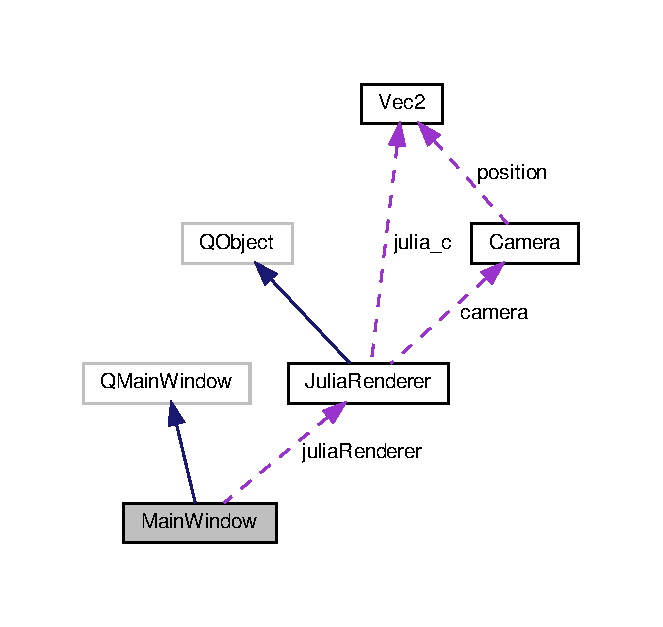
\includegraphics[width=318pt]{classMainWindow__coll__graph}
\end{center}
\end{figure}
\subsection*{Public Member Functions}
\begin{DoxyCompactItemize}
\item 
\hyperlink{classMainWindow_a996c5a2b6f77944776856f08ec30858d}{Main\+Window} (Q\+Widget $\ast$parent=nullptr)
\begin{DoxyCompactList}\small\item\em \hyperlink{classMainWindow}{Main\+Window} default construct. \end{DoxyCompactList}\item 
\hyperlink{classJuliaWidget}{Julia\+Widget} $\ast$ \hyperlink{classMainWindow_a7ee8a672f617c1eaa5a83b6db735e51b}{get\+Render\+Target} ()
\begin{DoxyCompactList}\small\item\em get\+Render\+Target pointer refered to class \hyperlink{classJuliaWidget}{Julia\+Widget} \end{DoxyCompactList}\item 
Q\+Label $\ast$ \hyperlink{classMainWindow_adc53673d5fb73e021c7bde51a3b32055}{get\+F\+PS} ()
\begin{DoxyCompactList}\small\item\em get\+F\+PS pointer refered to class Q\+Label \end{DoxyCompactList}\item 
int \hyperlink{classMainWindow_a60d21468b55f475cc6187e577f3237de}{get\+Value} ()
\begin{DoxyCompactList}\small\item\em get\+Value constructor \end{DoxyCompactList}\item 
double \hyperlink{classMainWindow_a53e364bc9d8029ce6cac0170985fca81}{get\+Imaginary} ()
\begin{DoxyCompactList}\small\item\em get\+Imaginary constructor \end{DoxyCompactList}\item 
double \hyperlink{classMainWindow_ac2e149fa1e1eacf3166c3fb6943a6623}{get\+Real} ()
\begin{DoxyCompactList}\small\item\em get\+Real construct \end{DoxyCompactList}\item 
int \hyperlink{classMainWindow_adfbd73af7cca6690ea0dc032d08770f2}{get\+Rendering\+Mode} ()
\begin{DoxyCompactList}\small\item\em get\+Rendering\+Mode constructor \end{DoxyCompactList}\item 
int \hyperlink{classMainWindow_ab882730b5ab7e570b52cddf7134a9e63}{get\+Color\+Mode} ()
\begin{DoxyCompactList}\small\item\em get\+Color\+Mode constructor \end{DoxyCompactList}\item 
void \hyperlink{classMainWindow_aadb538c3401816b2c6038696ca0f8628}{set\+Status\+Text} (Q\+String \&text)
\begin{DoxyCompactList}\small\item\em set\+Status\+Text constructor \end{DoxyCompactList}\item 
double \hyperlink{classMainWindow_a43d3aa3fbe5ea12500ad8933534a1424}{get\+Quality} ()
\begin{DoxyCompactList}\small\item\em get\+Quality constructor \end{DoxyCompactList}\end{DoxyCompactItemize}
\subsection*{Public Attributes}
\begin{DoxyCompactItemize}
\item 
\mbox{\Hypertarget{classMainWindow_a5b02344e17f89741b0ae69cdf9e9fcd2}\label{classMainWindow_a5b02344e17f89741b0ae69cdf9e9fcd2}} 
bool \hyperlink{classMainWindow_a5b02344e17f89741b0ae69cdf9e9fcd2}{resized} = false
\begin{DoxyCompactList}\small\item\em resized bool param initialised as false \end{DoxyCompactList}\item 
\mbox{\Hypertarget{classMainWindow_a089b453e1c44d35636f0b6f9d13605e3}\label{classMainWindow_a089b453e1c44d35636f0b6f9d13605e3}} 
bool \hyperlink{classMainWindow_a089b453e1c44d35636f0b6f9d13605e3}{exit\+Requested} = false
\begin{DoxyCompactList}\small\item\em exit\+Requested bool param initialised as false \end{DoxyCompactList}\item 
\mbox{\Hypertarget{classMainWindow_ac2778f4adcf69a9a707ff1ba88ece3f6}\label{classMainWindow_ac2778f4adcf69a9a707ff1ba88ece3f6}} 
\hyperlink{classJuliaRenderer}{Julia\+Renderer} $\ast$ \hyperlink{classMainWindow_ac2778f4adcf69a9a707ff1ba88ece3f6}{julia\+Renderer}
\begin{DoxyCompactList}\small\item\em julia\+Renderer pointer with class \hyperlink{classJuliaRenderer}{Julia\+Renderer} \end{DoxyCompactList}\end{DoxyCompactItemize}
\subsection*{Protected Member Functions}
\begin{DoxyCompactItemize}
\item 
void \hyperlink{classMainWindow_a2bb633e0547f37d75ba5ec77417b574f}{save\+Png} (int w, int h)
\begin{DoxyCompactList}\small\item\em save\+Png constructor \end{DoxyCompactList}\end{DoxyCompactItemize}


\subsection{Detailed Description}
The \hyperlink{classMainWindow}{Main\+Window} class Mainwindow include Qmainwindow. 

\subsection{Constructor \& Destructor Documentation}
\mbox{\Hypertarget{classMainWindow_a996c5a2b6f77944776856f08ec30858d}\label{classMainWindow_a996c5a2b6f77944776856f08ec30858d}} 
\index{Main\+Window@{Main\+Window}!Main\+Window@{Main\+Window}}
\index{Main\+Window@{Main\+Window}!Main\+Window@{Main\+Window}}
\subsubsection{\texorpdfstring{Main\+Window()}{MainWindow()}}
{\footnotesize\ttfamily Main\+Window\+::\+Main\+Window (\begin{DoxyParamCaption}\item[{Q\+Widget $\ast$}]{parent = {\ttfamily nullptr} }\end{DoxyParamCaption})\hspace{0.3cm}{\ttfamily [explicit]}}



\hyperlink{classMainWindow}{Main\+Window} default construct. 


\begin{DoxyParams}{Parameters}
{\em parent} & pointer as param \\
\hline
\end{DoxyParams}


\subsection{Member Function Documentation}
\mbox{\Hypertarget{classMainWindow_ab882730b5ab7e570b52cddf7134a9e63}\label{classMainWindow_ab882730b5ab7e570b52cddf7134a9e63}} 
\index{Main\+Window@{Main\+Window}!get\+Color\+Mode@{get\+Color\+Mode}}
\index{get\+Color\+Mode@{get\+Color\+Mode}!Main\+Window@{Main\+Window}}
\subsubsection{\texorpdfstring{get\+Color\+Mode()}{getColorMode()}}
{\footnotesize\ttfamily int Main\+Window\+::get\+Color\+Mode (\begin{DoxyParamCaption}{ }\end{DoxyParamCaption})}



get\+Color\+Mode constructor 

\begin{DoxyReturn}{Returns}
returning integer 
\end{DoxyReturn}
\mbox{\Hypertarget{classMainWindow_adc53673d5fb73e021c7bde51a3b32055}\label{classMainWindow_adc53673d5fb73e021c7bde51a3b32055}} 
\index{Main\+Window@{Main\+Window}!get\+F\+PS@{get\+F\+PS}}
\index{get\+F\+PS@{get\+F\+PS}!Main\+Window@{Main\+Window}}
\subsubsection{\texorpdfstring{get\+F\+P\+S()}{getFPS()}}
{\footnotesize\ttfamily Q\+Label$\ast$ Main\+Window\+::get\+F\+PS (\begin{DoxyParamCaption}{ }\end{DoxyParamCaption})}



get\+F\+PS pointer refered to class Q\+Label 

\begin{DoxyReturn}{Returns}
type get\+F\+PS 
\end{DoxyReturn}
\mbox{\Hypertarget{classMainWindow_a53e364bc9d8029ce6cac0170985fca81}\label{classMainWindow_a53e364bc9d8029ce6cac0170985fca81}} 
\index{Main\+Window@{Main\+Window}!get\+Imaginary@{get\+Imaginary}}
\index{get\+Imaginary@{get\+Imaginary}!Main\+Window@{Main\+Window}}
\subsubsection{\texorpdfstring{get\+Imaginary()}{getImaginary()}}
{\footnotesize\ttfamily double Main\+Window\+::get\+Imaginary (\begin{DoxyParamCaption}{ }\end{DoxyParamCaption})}



get\+Imaginary constructor 

\begin{DoxyReturn}{Returns}
returning double 
\end{DoxyReturn}
\mbox{\Hypertarget{classMainWindow_a43d3aa3fbe5ea12500ad8933534a1424}\label{classMainWindow_a43d3aa3fbe5ea12500ad8933534a1424}} 
\index{Main\+Window@{Main\+Window}!get\+Quality@{get\+Quality}}
\index{get\+Quality@{get\+Quality}!Main\+Window@{Main\+Window}}
\subsubsection{\texorpdfstring{get\+Quality()}{getQuality()}}
{\footnotesize\ttfamily double Main\+Window\+::get\+Quality (\begin{DoxyParamCaption}{ }\end{DoxyParamCaption})}



get\+Quality constructor 

\begin{DoxyReturn}{Returns}
returning double 
\end{DoxyReturn}
\mbox{\Hypertarget{classMainWindow_ac2e149fa1e1eacf3166c3fb6943a6623}\label{classMainWindow_ac2e149fa1e1eacf3166c3fb6943a6623}} 
\index{Main\+Window@{Main\+Window}!get\+Real@{get\+Real}}
\index{get\+Real@{get\+Real}!Main\+Window@{Main\+Window}}
\subsubsection{\texorpdfstring{get\+Real()}{getReal()}}
{\footnotesize\ttfamily double Main\+Window\+::get\+Real (\begin{DoxyParamCaption}{ }\end{DoxyParamCaption})}



get\+Real construct 

\begin{DoxyReturn}{Returns}
returning double 
\end{DoxyReturn}
\mbox{\Hypertarget{classMainWindow_adfbd73af7cca6690ea0dc032d08770f2}\label{classMainWindow_adfbd73af7cca6690ea0dc032d08770f2}} 
\index{Main\+Window@{Main\+Window}!get\+Rendering\+Mode@{get\+Rendering\+Mode}}
\index{get\+Rendering\+Mode@{get\+Rendering\+Mode}!Main\+Window@{Main\+Window}}
\subsubsection{\texorpdfstring{get\+Rendering\+Mode()}{getRenderingMode()}}
{\footnotesize\ttfamily int Main\+Window\+::get\+Rendering\+Mode (\begin{DoxyParamCaption}{ }\end{DoxyParamCaption})}



get\+Rendering\+Mode constructor 

\begin{DoxyReturn}{Returns}
returning integer 
\end{DoxyReturn}
\mbox{\Hypertarget{classMainWindow_a7ee8a672f617c1eaa5a83b6db735e51b}\label{classMainWindow_a7ee8a672f617c1eaa5a83b6db735e51b}} 
\index{Main\+Window@{Main\+Window}!get\+Render\+Target@{get\+Render\+Target}}
\index{get\+Render\+Target@{get\+Render\+Target}!Main\+Window@{Main\+Window}}
\subsubsection{\texorpdfstring{get\+Render\+Target()}{getRenderTarget()}}
{\footnotesize\ttfamily \hyperlink{classJuliaWidget}{Julia\+Widget} $\ast$ Main\+Window\+::get\+Render\+Target (\begin{DoxyParamCaption}{ }\end{DoxyParamCaption})}



get\+Render\+Target pointer refered to class \hyperlink{classJuliaWidget}{Julia\+Widget} 

\begin{DoxyReturn}{Returns}
type \hyperlink{classJuliaWidget}{Julia\+Widget} 
\end{DoxyReturn}
\mbox{\Hypertarget{classMainWindow_a60d21468b55f475cc6187e577f3237de}\label{classMainWindow_a60d21468b55f475cc6187e577f3237de}} 
\index{Main\+Window@{Main\+Window}!get\+Value@{get\+Value}}
\index{get\+Value@{get\+Value}!Main\+Window@{Main\+Window}}
\subsubsection{\texorpdfstring{get\+Value()}{getValue()}}
{\footnotesize\ttfamily int Main\+Window\+::get\+Value (\begin{DoxyParamCaption}{ }\end{DoxyParamCaption})}



get\+Value constructor 

\begin{DoxyReturn}{Returns}
returning integer 
\end{DoxyReturn}
\mbox{\Hypertarget{classMainWindow_a2bb633e0547f37d75ba5ec77417b574f}\label{classMainWindow_a2bb633e0547f37d75ba5ec77417b574f}} 
\index{Main\+Window@{Main\+Window}!save\+Png@{save\+Png}}
\index{save\+Png@{save\+Png}!Main\+Window@{Main\+Window}}
\subsubsection{\texorpdfstring{save\+Png()}{savePng()}}
{\footnotesize\ttfamily void Main\+Window\+::save\+Png (\begin{DoxyParamCaption}\item[{int}]{w,  }\item[{int}]{h }\end{DoxyParamCaption})\hspace{0.3cm}{\ttfamily [protected]}}



save\+Png constructor 


\begin{DoxyParams}{Parameters}
{\em w} & integer param \\
\hline
{\em h} & integer param \\
\hline
\end{DoxyParams}
\mbox{\Hypertarget{classMainWindow_aadb538c3401816b2c6038696ca0f8628}\label{classMainWindow_aadb538c3401816b2c6038696ca0f8628}} 
\index{Main\+Window@{Main\+Window}!set\+Status\+Text@{set\+Status\+Text}}
\index{set\+Status\+Text@{set\+Status\+Text}!Main\+Window@{Main\+Window}}
\subsubsection{\texorpdfstring{set\+Status\+Text()}{setStatusText()}}
{\footnotesize\ttfamily void Main\+Window\+::set\+Status\+Text (\begin{DoxyParamCaption}\item[{Q\+String \&}]{text }\end{DoxyParamCaption})}



set\+Status\+Text constructor 


\begin{DoxyParams}{Parameters}
{\em text} & param defined as reference \\
\hline
\end{DoxyParams}


The documentation for this class was generated from the following files\+:\begin{DoxyCompactItemize}
\item 
mainwindow.\+h\item 
mainwindow.\+cpp\end{DoxyCompactItemize}

\hypertarget{classVec2}{}\section{Vec2 Class Reference}
\label{classVec2}\index{Vec2@{Vec2}}


The \hyperlink{classVec2}{Vec2} class (x,y)  




{\ttfamily \#include $<$vec2.\+h$>$}

\subsection*{Public Member Functions}
\begin{DoxyCompactItemize}
\item 
\mbox{\Hypertarget{classVec2_a76080feed7005893ecc634f903cfbae0}\label{classVec2_a76080feed7005893ecc634f903cfbae0}} 
\hyperlink{classVec2_a76080feed7005893ecc634f903cfbae0}{Vec2} ()
\begin{DoxyCompactList}\small\item\em \hyperlink{classVec2}{Vec2} konstructor default, x,y = 0. \end{DoxyCompactList}\item 
\hyperlink{classVec2_a01363a5456ac9b4a9b92cb6b7d7eb82a}{Vec2} (double \hyperlink{classVec2_a0ee7118259bcfc2fe997d4bf816ed682}{x}, double \hyperlink{classVec2_a9c6f37b5242919bccff799c8f05dee55}{y})
\begin{DoxyCompactList}\small\item\em \hyperlink{classVec2}{Vec2} with two parameters. \end{DoxyCompactList}\item 
void \hyperlink{classVec2_a3574fcb9ccc0abd7e7e82abe22dabb83}{set} (double \hyperlink{classVec2_a0ee7118259bcfc2fe997d4bf816ed682}{x}, double \hyperlink{classVec2_a9c6f37b5242919bccff799c8f05dee55}{y})
\begin{DoxyCompactList}\small\item\em set actual Position \end{DoxyCompactList}\item 
void \hyperlink{classVec2_a591966ea1b13cf9333e57999e4953465}{add} (double \hyperlink{classVec2_a0ee7118259bcfc2fe997d4bf816ed682}{x}, double \hyperlink{classVec2_a9c6f37b5242919bccff799c8f05dee55}{y})
\begin{DoxyCompactList}\small\item\em add methode, algorith for calculate camera position \end{DoxyCompactList}\item 
double \hyperlink{classVec2_a0cf7a6aad8f6b48805455f31a69feb5d}{get\+Length} ()
\begin{DoxyCompactList}\small\item\em get\+Length Length of vector \end{DoxyCompactList}\item 
double \hyperlink{classVec2_a229954458b6789250afb7f6af143002c}{get\+Length\+Squared} ()
\begin{DoxyCompactList}\small\item\em get\+Length\+Squared Squared lenght of vector \end{DoxyCompactList}\end{DoxyCompactItemize}
\subsection*{Public Attributes}
\begin{DoxyCompactItemize}
\item 
\mbox{\Hypertarget{classVec2_a0ee7118259bcfc2fe997d4bf816ed682}\label{classVec2_a0ee7118259bcfc2fe997d4bf816ed682}} 
double \hyperlink{classVec2_a0ee7118259bcfc2fe997d4bf816ed682}{x}
\begin{DoxyCompactList}\small\item\em x variable \end{DoxyCompactList}\item 
\mbox{\Hypertarget{classVec2_a9c6f37b5242919bccff799c8f05dee55}\label{classVec2_a9c6f37b5242919bccff799c8f05dee55}} 
double \hyperlink{classVec2_a9c6f37b5242919bccff799c8f05dee55}{y}
\begin{DoxyCompactList}\small\item\em y variable \end{DoxyCompactList}\end{DoxyCompactItemize}


\subsection{Detailed Description}
The \hyperlink{classVec2}{Vec2} class (x,y) 

\subsection{Constructor \& Destructor Documentation}
\mbox{\Hypertarget{classVec2_a01363a5456ac9b4a9b92cb6b7d7eb82a}\label{classVec2_a01363a5456ac9b4a9b92cb6b7d7eb82a}} 
\index{Vec2@{Vec2}!Vec2@{Vec2}}
\index{Vec2@{Vec2}!Vec2@{Vec2}}
\subsubsection{\texorpdfstring{Vec2()}{Vec2()}}
{\footnotesize\ttfamily Vec2\+::\+Vec2 (\begin{DoxyParamCaption}\item[{double}]{x,  }\item[{double}]{y }\end{DoxyParamCaption})}



\hyperlink{classVec2}{Vec2} with two parameters. 


\begin{DoxyParams}{Parameters}
{\em x} & position x \\
\hline
{\em y} & position y \\
\hline
\end{DoxyParams}


\subsection{Member Function Documentation}
\mbox{\Hypertarget{classVec2_a591966ea1b13cf9333e57999e4953465}\label{classVec2_a591966ea1b13cf9333e57999e4953465}} 
\index{Vec2@{Vec2}!add@{add}}
\index{add@{add}!Vec2@{Vec2}}
\subsubsection{\texorpdfstring{add()}{add()}}
{\footnotesize\ttfamily void Vec2\+::add (\begin{DoxyParamCaption}\item[{double}]{x,  }\item[{double}]{y }\end{DoxyParamCaption})}



add methode, algorith for calculate camera position 


\begin{DoxyParams}{Parameters}
{\em x} & postion x \\
\hline
{\em y} & position y \\
\hline
\end{DoxyParams}
\mbox{\Hypertarget{classVec2_a0cf7a6aad8f6b48805455f31a69feb5d}\label{classVec2_a0cf7a6aad8f6b48805455f31a69feb5d}} 
\index{Vec2@{Vec2}!get\+Length@{get\+Length}}
\index{get\+Length@{get\+Length}!Vec2@{Vec2}}
\subsubsection{\texorpdfstring{get\+Length()}{getLength()}}
{\footnotesize\ttfamily double Vec2\+::get\+Length (\begin{DoxyParamCaption}{ }\end{DoxyParamCaption})}



get\+Length Length of vector 

\begin{DoxyReturn}{Returns}
returning double 
\end{DoxyReturn}
\mbox{\Hypertarget{classVec2_a229954458b6789250afb7f6af143002c}\label{classVec2_a229954458b6789250afb7f6af143002c}} 
\index{Vec2@{Vec2}!get\+Length\+Squared@{get\+Length\+Squared}}
\index{get\+Length\+Squared@{get\+Length\+Squared}!Vec2@{Vec2}}
\subsubsection{\texorpdfstring{get\+Length\+Squared()}{getLengthSquared()}}
{\footnotesize\ttfamily double Vec2\+::get\+Length\+Squared (\begin{DoxyParamCaption}{ }\end{DoxyParamCaption})}



get\+Length\+Squared Squared lenght of vector 

\begin{DoxyReturn}{Returns}
returning double 
\end{DoxyReturn}
\mbox{\Hypertarget{classVec2_a3574fcb9ccc0abd7e7e82abe22dabb83}\label{classVec2_a3574fcb9ccc0abd7e7e82abe22dabb83}} 
\index{Vec2@{Vec2}!set@{set}}
\index{set@{set}!Vec2@{Vec2}}
\subsubsection{\texorpdfstring{set()}{set()}}
{\footnotesize\ttfamily void Vec2\+::set (\begin{DoxyParamCaption}\item[{double}]{x,  }\item[{double}]{y }\end{DoxyParamCaption})}



set actual Position 


\begin{DoxyParams}{Parameters}
{\em x} & position x \\
\hline
{\em y} & position y \\
\hline
\end{DoxyParams}


The documentation for this class was generated from the following files\+:\begin{DoxyCompactItemize}
\item 
vec2.\+h\item 
vec2.\+cpp\end{DoxyCompactItemize}

%--- End generated contents ---

% Index
\backmatter
\newpage
\phantomsection
\clearemptydoublepage
\addcontentsline{toc}{chapter}{Index}
\printindex

\end{document}
